\section{Zahlenfolgen}

\[
	\langle a_n \rangle = a_1,\ a_2,\ a_3,\ a_4,\ \ldots,\ a_n \quad n \in \mathbb{N},\ a : \mathbb{N} \rightarrow \mathbb{R}
\]

\subsection{Allgemeines Bildungsgesetz}

\paragraph{explizite Darstellungsform}

\[
	a_n = f(n)
\]

\paragraph{rekursive Darstellungsform}

\begin{align*}
	a_{n+1} & = F(a_n)          \\
	a_{n+1} & = F(a_n, a_{n-1})
\end{align*}

\subsection{Die harmonische Folge}

\[
	a_n = f(n) = \frac{1}{n}
\]

\[
	\langle a_n \rangle = 1,\ \frac{1}{2},\ \frac{1}{3},\ \frac{1}{4},\ \frac{1}{5},\ \ldots,\ \frac{1}{n}
\]

\subsection{Arithmetische Folgen}

\subsubsection{Bildungsgesetz}

\begin{align*}
	a_n     & = \frac{a_{n+1} + a_{n-1}}{2} \\
	2 a_n   & = a_{n+1} + a_{n-1}           \\
	a_{n+1} & = 2 a_n - a_{n-1}
\end{align*}

\begin{gesetz}
	\paragraph{Rekursives Bildungsgesetz}

	\[
		a_{n+1} = 2 a_n - a_{n-1}
	\]
\end{gesetz}

\paragraph{Beispiel}

\subparagraph{Anfangsbedingung:}

\begin{align*}
	a_1 & = a     \\
	a_2 & = a + d
\end{align*}

\[
	\begin{alignedat}{4}
		a_3 & : a_{2+1} & = 2a_2 - a_1 & \Rightarrow a_3 = 2(a+d) - a       & = a + 2d \\
		a_4 & : a_{3+1} & = 2a_3 - a_2 & \Rightarrow a_4 = 2(a+2d) - (a+d)  & = a + 3d \\
		a_5 & : a_{4+1} & = 2a_4 - a_3 & \Rightarrow a_4 = 2(a+3d) - (a+2d) & = a + 4d
	\end{alignedat}
\]


\begin{gesetz}
	\paragraph{Explizites Bildungsgesetz}

	\[
		a_n = a + (n - 1)d
	\]
\end{gesetz}

\subsubsection{Beispiel für eine Folge 1. Ordnung}

\[
	\langle a_n \rangle = 6 \underbrace{,}_{4} 10 \underbrace{,}_{4} 14 \underbrace{,}_{4} 18,\ \ldots \\
\]

\paragraph{Allgemeine Lösung}

\[
	a_n = c_1 \cdot n + c_2 \\
\]

\paragraph{Lösungsweg}

\begin{align*}
	\left.
	\begin{array}{l}
		6 = c_1 \cdot 1 + c_2 \\
		10 = c_1 \cdot 2 + c_2
	\end{array}
	\right \}
	\left.
	\begin{array}{l}
		c_1 = 4 \\
		c_2 = 2
	\end{array}
	\right.
\end{align*}

\paragraph{Lösung}

\[
	*a_n = 6 + (n - 1) \cdot 4 = 2 + 4 n
\]

\subsubsection{Beispiel für eine Folge 2. Ordnung}

\[
	\langle a_n \rangle = 1,\ 7,\ 17,\ 31,\ 49,\ \ldots
\]

\[
	\begin{tabular}{ccccccccccccc}
		1 & ,    & 7    & ,    & 17   & ,    & 31   & ,    & 49 \\[-3pt]
		  & \ubf &      & \ubf &      & \ubf &      & \ubf      \\
		  & 6    &      & 10   &      & 14   &      & 18        \\[-3pt]
		  &      & \ubf &      & \ubf &      & \ubf             \\
		  &      & 4    &      & 4    &      & 4
	\end{tabular}
\]

\paragraph{Allgemeine Lösung}

\[
	a_n = c_1\ n^2 + c_2\ n + c_3
\]

\paragraph{Lösungsweg}

\[
	\left.
	\begin{array}{lcl}
		1  & = c_1 \cdot 1^2 + c_2 \cdot 1 + c_3 \\
		7  & = c_1 \cdot 2^2 + c_2 \cdot 2 + c_3 \\
		17 & = c_1 \cdot 3^2 + c_2 \cdot 3 + c_3
	\end{array}
	\right \}
	a_n = 2n^2 {-} 1
\]

\subsection{Gaußscher Algorithmus}

\begin{align*}
    \sum_{i=1}^n a_i &= a_1 + a_2 + a_3 + \cdots + a_{n-1} + a_n \\
    \\
    \sum_{i=1}^n a_i &= a + (a + d) + (a + 2d) + \cdots + (a +(n-2) d) + (a + (n - 1) d) \\
    \sum_{i=1}^n a_i &= (a + (n-1)d) + (a +(n-2) d) + \cdots + (a + 2d) + (a + d) + a \\
    \cline{1-2}
    2 \cdot \sum_{i=1}^n a_i &= (2a+(n-1)d) + (2a+(n-1)d) + \cdots + (2a+(n-1)d) \\
    \\
    2 \cdot \sum_{i=1}^n a_i &= n (2a+(n-1)d) = 2n a + n(n-1)d
\end{align*}

\begin{gesetz}
    \paragraph{Summe einer arithmetischen Folge bis \(n\)}
    \[
        \sum_{i=1}^n a_i = n a + \frac{n(n-1)}{2} d
    \]
\end{gesetz}

\subsection{Geometrische Folgen}

\subsubsection{Bildungsgesetz}

\begin{align*}
	a_n   & = \sqrt{a_{n+1} \cdot a_{n-1}} \\
	a_n^2 & = a_{n+1} \cdot a_{n-1}
\end{align*}

\begin{gesetz}
	\paragraph{Rekursives Bildungsgesetz}
	\[
		a_{n+1} = \frac{a_n^2}{a_{n-1}}
	\]
\end{gesetz}

\begin{align*}
	a_1 & = a                                                 \\
	a_2 & = a \cdot q                                         \\
	a_3 & = \frac{{(a \cdot q)}^2}{a} = a \cdot q^2           \\
	a_4 & = \frac{{(a \cdot q^2)}^2}{a \cdot q} = a \cdot q^3
\end{align*}

\begin{gesetz}
	\paragraph{Explizites Bildungsgesetz}
	\[
		a_n = a \cdot q^{n-1}
	\]
\end{gesetz}

\[
	q = \frac{a_{n+1}}{a_n}
\]

\subsubsection{Summe einer geometrischen Folge}

\[
	\begin{array}{ccccccccc}
		q \cdot S_n       & = &                                           & a q^1         & + a q^2  & + a q^3 & + \cdots & + a q^{n-1} & + a q^n \\
		S_n               & = & a                                         & + a q^1       & + a  q^2 & + a q^3 & + \cdots & + a q^{n-1} &         \\
		\cline{1-9}
		q \cdot S_n - S_n & = & -a                                        & + a \cdot a^n &          &         &          &             &         \\
		S_n(q-1)          & = & a(q^n -1)                                 &               &          &         &          &             &         \\
		S_n               & = & a \cdot \frac{q^n - 1}{q - 1}             &               &          &         &          &             &         \\
		                  & = & a \cdot \frac{(q^n - 1)(-1)}{(q - 1)(-1)} &               &          &         &          &             &         \\
		                  & = & a \cdot \frac{1- q^n}{1 - q}              &               &          &         &          &             &         \\
	\end{array}
\]

\begin{gesetz}
	\paragraph{Summe einer geometrischen Folge bis \(n\)}
	\[
		S_n = a \cdot \frac{1 - q^n}{1 - q}
	\]
\end{gesetz}

\paragraph{1. Fall: \(q > 1, a > 0\)}

\[
	S_n \rightarrow \infty
\]

\paragraph{2. Fall: \(0 < q < 1, a > 0\)}

\[
	S_n = a \cdot \frac{1}{1-q}
\]

\subsection{Übungsaufgaben}

\begin{uebung}
	\begin{question}
		\[
			\langle a_n \rangle = 1,\ 6,\ 11,\ 16,\ 21,\ \ldots
		\]
	\end{question}

	\begin{solution}
		\[
			1\underbrace{\quad}_{5}6\underbrace{\quad}_{5}11\underbrace{\quad}_{5}16\underbrace{\quad}_{5}21
		\]
		\[
			a_n = 1+(5n - 1) = 5n - 4
		\]
	\end{solution}

	\begin{question}
		\[
			\langle a_n \rangle = 5,\ 11,\ 21,\ 35,\ 53,\ \ldots
		\]
	\end{question}

	\begin{solution}
		\[
			\begin{tabular}{ccccccccccccc}
				5 &      & 11   &      & 21   &      & 35   &      & 53 \\[-3pt]
				  & \ubf &      & \ubf &      & \ubf &      & \ubf      \\
				  & 6    &      & 10   &      & 14   &      & 18        \\[-3pt]
				  &      & \ubf &      & \ubf &      & \ubf             \\
				  &      & 4    &      & 4    &      & 4
			\end{tabular}
		\]
		\[
			a_n = c_1 \cdot n^2 + c_2 \cdot n + c_3 \\
		\]
		\begin{align*}
			\left.
			\begin{array}{ccccc}
				5  & = 1 c_1 & + 1 c_2 & + c_3 \\
				11 & = 4 c_1 & + 2 c_2 & + c_3 \\
				21 & = 9 c_1 & + 3 c_2 & + c_3
			\end{array}
			\right \}
			\left.
			\begin{array}{cc}
				c_1 & = 2 \\
				c_2 & = 0 \\
				c_3 & = 3
			\end{array}
			\right \}
			a_n = 2n^2 + 3
		\end{align*}
	\end{solution}

	\begin{question}
		\[
			\langle a_n \rangle = \frac{2}{1!},\ \frac{5}{2!},\ \frac{8}{3!},\ \frac{11}{4!},\ \frac{14}{5!},\ \ldots
		\]
	\end{question}

	\begin{solution}
		\subparagraph{Nenner}
		\[
			a_n = \frac{x}{n!}
		\]
		\subparagraph{Zähler}
		\[
			\begin{tabular}{ccccccccccccc}
				   & 3    &    & 3    &    & 3    &    & 3                  \\[-3pt]
				   & \obf &    & \obf &    & \obf &    & \obf               \\
				2  &      & 5  &      & 8  &      & 11 &      & 14          \\
				\cline{1-1} \cline{3-3} \cline{5-5} \cline{7-7} \cline{9-9} \\[-10pt]
				1! &      & 2! &      & 3! &      & 4! &      & 5!          \\
			\end{tabular}
		\]
		\[
			x = 2 + (n-1) 3 = 3n - 1
		\]
		\[
			a_n = \frac{3n - 1}{n!}
		\]
	\end{solution}
\end{uebung}

\subsection{Rekursionsschnecke}

\begin{figure}[H]
	\centering
    \includegraphics[scale=0.8]{grafiken/Rekursionsschnecke.eps}
	\caption{Die \enquote{Rekursionsschnecke}}\label{fig:rekusionsschnecke}
\end{figure}

\paragraph{Aufgabe 1}

\[
    a_n =\ ?
\]

\paragraph{Lösungsweg}

\subparagraph{Satz des Pythagoras}

\begin{align*}  
    a_1^2 + a_1^2 &= D^2 \\
    2 a_1^2 &= 10^2 \\
    a_1^2 &= 50 \\
    a_1 &= \sqrt{50}
\end{align*}

\begin{align*}
    a_2^2 + a_2^2 &= a_1^2 \\
    2 a_2^2 &= {\sqrt{50}}^2 \\
    a_2^2 &= \frac{50}{2} \\
    a_2 &= \sqrt{\frac{50}{2}} = \sqrt{50} \cdot \frac{1}{\sqrt{2}}
\end{align*}

\begin{align*}
    a_3^2 + a_3^2 &= a_2^2 \\
    2 a_3^2 &= \frac{50}{2} \\
    a_3^2 &= \frac{50}{4} \\
    a_3 &= \sqrt{50} \cdot \frac{1}{\sqrt{4}}
\end{align*}

\[
    \langle a_n \rangle = \sqrt{50},\ \sqrt{50} \cdot \frac{1}{\sqrt{2}},\ \sqrt{50} \cdot \frac{1}{\sqrt{4}},\ \ldots \
\]

\subparagraph{geometrische Folge}

\begin{align*}
    a_n &= a \cdot q^{n-1} \\
    a_n &= \sqrt{50} \cdot \sqrt{\frac{1}{2^{n-1}}} \\
    &= \sqrt{50} \cdot {\left(\frac{1}{\sqrt{2}}\right)}^{n-1} \\
    \Rightarrow q &= \frac{1}{\sqrt{2}}
\end{align*}

\paragraph{Aufgabe 2}

\[
    S =\ ?
\]

\paragraph{Lösungsweg}

\[
    S = a \cdot \frac{1 - q^n}{1 - q} = \sqrt{50} \cdot \frac{1}{1- \frac{1}{\sqrt{2}}} \approx 24,14
\]

